\documentclass[a4paper,openany]{book}
\usepackage[a4paper,left=2cm,right=2cm,top=0.5cm,bottom=0.5cm,includehead,includefoot,headheight=0.1cm,heightrounded]{geometry}
\usepackage{amsmath}
\usepackage{graphics}
\usepackage{graphicx}
\usepackage[table,xcdraw]{xcolor}
\usepackage{float}
\usepackage[pro]{fontawesome5}
\usepackage{ragged2e}
\usepackage{titlesec}
\usepackage{tikz}
\usepackage[export]{adjustbox}
\usepackage{tocloft}
\usepackage{etoolbox}
\renewcommand{\contentsname}{\normalfont \sffamily \huge \textcolor{id7-aubergine}{Table of Contents}\vspace{-1.25em}}
\renewcommand{\cftsecfont}{\normalfont}
\renewcommand{\cftsecpagefont}{\normalfont}
\usetikzlibrary{automata, positioning, shapes.symbols, arrows, chains, calc}
\usepackage{shellesc}
\usepackage{minted}
\usepackage{listings}
\usepackage[hidelinks]{hyperref}
%\usepackage[osfigures]{opensans}
\usepackage{lastpage}
\usepackage{fancyhdr}
\usepackage{mdframed}
\usepackage{outlines}
\usepackage{bm}
\usepackage{array}
\usepackage{enumitem}
\usepackage[round]{natbib}
\usepackage{environ}
\usepackage{varwidth}
\usepackage{mathtools}
\usepackage{pagecolor}
\usepackage{wrapfig}
\usepackage{nameref}
\usepackage{fontspec}
\setsansfont{Proxima Nova}
\newfontfamily\warwickfont[
Scale=MatchLowercase
%  Path = fonts/
]{Avenir Next}
\makeatletter
\newcommand*{\currentname}{\@currentlabelname}
\makeatother
\usepackage{csquotes}
\usepackage{newfloat}
\usepackage{caption}
\usepackage[super]{nth}
\titleformat{\chapter}[display]
{\normalfont \sffamily \Huge  \color{id7-aubergine}}
{\vspace{-20pt} \flushright \large \color{id7-aubergine} \warwickfont \MakeUppercase { \chaptertitlename \hspace{1 ex} }  { \fontsize{60}{60}\selectfont \color{id7-aubergine} \sffamily  \thechapter }} {0 pt}{\vspace{-40pt}\Huge}
\newlength{\MyMdframedWidthTweak}%
\NewEnviron{MyMdframed}[1][]{%
    \setlength{\MyMdframedWidthTweak}{\dimexpr%
        +\mdflength{innerleftmargin}
        +\mdflength{innerrightmargin}
        +\mdflength{leftmargin}
        +\mdflength{rightmargin}
    }%
    \savebox0{%
        \begin{varwidth}{\dimexpr\linewidth-\MyMdframedWidthTweak\relax}%
            \BODY
        \end{varwidth}%
    }%
    \begin{mdframed}[
        backgroundcolor=lightgrey,
        topline=true,
        rightline=false,
        leftline=false,
        linecolor=id7-aubergine,
        userdefinedwidth=\dimexpr\wd0+\MyMdframedWidthTweak\relax, 
        #1]
        \usebox0
    \end{mdframed}
}
\titlespacing*{\chapter}
{0pt}{0pt}{2.0ex}
\DeclarePairedDelimiter\abs{\lvert}{\rvert}%
\title{}
\author{}
\definecolor{infogreen}{rgb}{0.153, 0.682, 0.376}
\definecolor{id7-aubergine}{HTML}{5B3069}
\definecolor{id7-gray}{HTML}{3F4246}
\definecolor{body-text}{HTML}{333333}
\definecolor{id7-gold}{HTML}{886C11}
\definecolor{id7-burnt-orange}{HTML}{A14418}
\definecolor{id7-ruby-red}{HTML}{89102C}
\definecolor{id7-emerald-green}{HTML}{797906}
\definecolor{id7-sky-blue}{HTML}{204F79}
\definecolor{id7-sky-blue-tint}{HTML}{bccad7}
\definecolor{skyblue}{rgb}{0.125, 0.31, 0.475}
\setlength{\parindent}{0em}
\setlength{\parskip}{1em}
\definecolor{todocolor}{rgb}{0.688,0.8176,0.93137}
\newcommand{\todobox}[1] {\colorbox{todocolor}{\parbox{\textwidth}{\vspace{.75\baselineskip}\centering\parbox{0.95\textwidth}{\faicon{lightbulb-o} \textbf{TODO:} #1\vspace{.75\baselineskip}}}}}
\newcommand{\readbox}[1] {\colorbox{infogreen}{\parbox{\textwidth}{\vspace{.75\baselineskip}\centering\parbox{0.95\textwidth}{\textcolor{white}{\faicon{book} \textbf{#1}\vspace{.75\baselineskip}}}}}}
\def\labelitemi{\textcolor{id7-aubergine}{\textbullet}}
\def\labelitemii{\textcolor{id7-aubergine}{\circ}}
\def\labelitemiii{\textcolor{id7-aubergine}{--}}
\definecolor{infogreenlight}{rgb}{0.75,1,0.75}

\newcommand{\infobox}[1] {\colorbox{infogreenlight}{\parbox{\textwidth}{\vspace{.75\baselineskip}\centering\parbox{0.95\textwidth}{\faicon{info-circle} #1\vspace{.75\baselineskip}}}}}

\newcommand{\boxedfigure}[2]{\begin{MyMdframed}\begin{figure}[H]
            \begin{center}\vspace{2em}\includegraphics[width=0.5\textwidth]{#1}\end{center}
            \caption{#2}
\end{figure}\end{MyMdframed}}

\newcommand{\widthboxedfigure}[3]{\begin{MyMdframed}\begin{figure}[H]
            \begin{center}\vspace{2em}\includegraphics[width=#3\textwidth]{#1}\end{center}
            \caption{#2}
\end{figure}\end{MyMdframed}}

\newcommand{\infoinlineicon}[1] {\colorbox{infogreenlight}{\faicon{info-circle} #1}}

\newcommand{\infoinline}[1] {\colorbox{infogreenlight}{#1}}

\definecolor{orange}{rgb}{0.9529,0.85176,0.5070588}

\newcommand{\warnbox}[1] {\colorbox{orange}{\parbox{\textwidth}{\vspace{.75\baselineskip}\centering\parbox{0.95\textwidth}{\faicon{exclamation-triangle} #1\vspace{.75\baselineskip}}}}}

\newcommand{\warninlineicon}[1] {\colorbox{orange}{\faicon{exclamation-triangle} #1}}

\makeatletter
\let\old@rule\@rule
\def\@rule[#1]#2#3{\textcolor{lightgrey}{\old@rule[#1]{#2}{#3}}}
\makeatother

\newcommand{\warninline}[1] {\colorbox{orange}{#1}}

\titleformat{\section}
{\normalfont\sffamily\huge\color{id7-aubergine}}
{\thesection. }{0em}{}

\titleformat{\subsection}
{\normalfont\Large\sffamily\color{id7-aubergine}}
{\thesubsection. }{0em}{}

\titleformat{\subsubsection}
{\normalfont\large\sffamily\color{id7-aubergine}}
{\thesubsubsection. }{0em}{}
\fancyhf{}
\pagestyle{fancy}

\renewcommand{\headrulewidth}{0pt}
\lfoot{\textcolor{grey}{Adam Williams}}
\rfoot{\textcolor{grey}{Page \thepage{} of \pageref{LastPage}}}

\renewcommand*\footnoterule{\noindent\makebox[\textwidth]{\includegraphics[width=\paperwidth]{divider}}}

% Redefine the plain page style
\fancypagestyle{plain}{%
	\fancyhf{}%
	\fancyhead[L]{\textcolor{grey}{\thedate}}%
	\fancyhead[R]{\textcolor{grey}{\currentname}}%
	\fancyfoot[L]{\textcolor{grey}{Adam Williams}}%
	\fancyfoot[R]{\textcolor{grey}{Page \thepage{} of \pageref{LastPage}}}%
	\renewcommand{\headrulewidth}{0pt}% Line at the header invisible
	\renewcommand{\footrulewidth}{0pt}% Line at the footer visible
}
\definecolor{grey}{rgb}{0.5,0.5,0.5}
\definecolor{lightgrey}{rgb}{0.96,0.96,0.96}

\def \spacedrule {\textcolor{id7-aubergine}{\hrule}\vspace{1em}}
\def \thedate {\today}
\lhead{\textcolor{grey}{\thedate}}
\rhead{\textcolor{grey}{\currentname}}

% Set up example boxes

\DeclareFloatingEnvironment[fileext=frm,placement={!ht},name=Example]{exampleflt}
\captionsetup[exampleflt]{labelfont=bf}

\newenvironment{example}[1]
{\begin{exampleflt}[tb]
		\begin{mdframed}
			\captionsetup{name=\faPuzzlePiece{} Example, singlelinecheck=false,font={color=id7-aubergine,sf},position=top}
			\vspace{0.5em}
			 \caption{#1}\hfill 
			\rmfamily
			\captionsetup{style=default}

			}
			{\end{mdframed}\end{exampleflt}
}

% And algorithm boxes

\DeclareFloatingEnvironment[fileext=frm,placement={!ht},name=Algorithm]{algorithmflt}
\captionsetup[figure]{name=\faImage{} Figure, singlelinecheck=false,font={color=id7-aubergine,sf},position=top,labelfont=bf}

\newenvironment{algbox}[1]
{\begin{algorithmflt}[tb]
		\begin{mdframed}
			\captionsetup{name=\faCogs{} Algorithm, singlelinecheck=false,font={color=id7-aubergine,sf},position=top}
			\vspace{0.5em}
			\caption{#1}\hfill 
			\rmfamily
			\captionsetup{style=default}
			
		}
		{\end{mdframed}\end{algorithmflt}
}

% And code boxes

\DeclareFloatingEnvironment[fileext=frm,placement={!ht},name=Code Listing]{codeflt}
\captionsetup[algorithmflt]{labelfont=bf}
\captionsetup[figure]{labelfont=bf}
\renewcommand{\theFancyVerbLine}{\rmfamily \textcolor[rgb]{0.7, 0.7, 0.7}{\arabic{FancyVerbLine}}}

\newenvironment{mycode}[4][]
{\VerbatimEnvironment
	\begin{codeflt}[tb]\begin{mdframed}
		\captionsetup{name=\faIcon{brackets-curly} \textbf{Code Listing}, singlelinecheck=false,font={color=id7-aubergine,sf},position=top}
		\vspace{0.5em}
		\caption{#3 \hfill #4}
		\vspace{0.5em}
		\captionsetup{style=default} 
	\begin{minted}[#1]{#2}}
	{\end{minted}\vspace{0.5em}\end{mdframed}\end{codeflt}}

\newenvironment{mycodefile}[5][]
{
	\begin{codeflt}[tb]\begin{mdframed}
			\captionsetup{name=\faIcon{brackets-curly} \textbf{Code Listing}, singlelinecheck=false,font={color=id7-aubergine,sf},position=top}
			\vspace{0.5em}
			\caption{#3 \hfill #4}
			\vspace{0.5em}
			\captionsetup{style=default} 
			\inputminted{#2}{#5}}
			{\vspace{0.5em}\end{mdframed}\end{codeflt}}
	
% ======================

\begin{document}
  
\newgeometry{margin=0in}
\begin{titlepage}
    
    \tikz[remember picture,overlay] \node[opacity=1,inner sep=0pt] at (current page.center){
\includegraphics[width=\paperwidth,height=\paperheight]{bg.eps}};
    \vspace{0.666\textheight} % height of the devil
    
    {\hspace{0pt}\vspace{0pt}\begin{tikzpicture}[scale=\paperwidth/1cm, overlay]
        \filldraw[draw=none,fill=white]
        (0, 0)
        -- (0.65838,0) 
        -- (0.71534285714,-0.1) 
        -- (0.7577,-0.0215)
        -- (0.8001, -0.1)
        -- (0.8571,0)
        -- (1, 0)
        -- (1, -0.45)
        -- (0, -0.45);
        
        \node[opacity=1,inner sep=0pt] at (0.7577, -0.15){
\includegraphics[width=6cm]{logotype}};
        \node[text width=15cm] at (0.39,-0.15) {\warwickfont\fontsize{40}{10}\selectfont\textcolor{id7-aubergine}{Regular Expression\\\vspace{0.2cm}Refinement Types}};
        \end{tikzpicture}}
    
    {\par}
    \vspace{1.25cm}
    \vspace{3.5cm}
    {\hspace{0.75cm}\Huge \warwickfont Project Report}
    \vspace{0.16cm}
    {\par}
    {\hspace{0.75cm}\large \warwickfont Adam Williams (3\textsuperscript{rd} year Computer Science)}


    {\hspace{0.75cm}\large \warwickfont Michael Gale (supervisor)}
    \vfill
\end{titlepage}
\restoregeometry
\restorepagecolor

\pagebreak[5]
\newenvironment{abstract}{\centering{\normalfont\Large\sffamily\color{id7-aubergine}Abstract}\vspace{0.3cm}\\
	\hfill\begin{minipage}{0.95\textwidth}
		\rule{\textwidth}{1pt}}
	{\par\noindent\rule{\textwidth}{1pt}\end{minipage}}

\begin{abstract}
	Entire classes of modern web application vulnerabilities arise due to problematic user input handling. This includes cross-site scripting (XSS), \emph{injection} issues (SQL, LDAP, etc), insecure
	deserialisation and file inclusion vulnerabilities – all of which are encountered by information
	security firms on a regular basis in application assessments. This project explores the use of regular expressions as refinement types for constrained data in order to model user input validation. We
	normalise the type system of such a language and implement it. We then compare our system to and evaluate it against other, existing approaches by considering false positive and negative rates with a
	series of test cases. 
\end{abstract}

\tableofcontents


\chapter{Motivation}

\section{Application Security}

\begin{itemize}
	\item What is it?
	\item Example vulnerabilities
	\item Case studies, impact
\end{itemize}

\section{Static Analysis}

\begin{itemize}
	\item Why static analysis over runtime/dynamic analysis?
	\item SAST/DAST
	\item Benefits for developers
\end{itemize}


\chapter{Background}
This chapter discusses the theory underpinning the techniques used in the implementation.


\section{Regular Expressions}

Most programming languages include support for using \emph{regular expressions} to match strings. Formally, regular expressions are a means to specify a \emph{regular} language -- equivalent in power to the \emph{deterministic finite automaton} (DFA) and \emph{non-deterministic finite automaton} (NFA).



Some (or all) of the following operations are available to use when building a recognising a language using regular expressions:

\begin{description}
	\item[$R^*$ (Kleene-star)] Accept zero or more of the expression $R$.
	\item[$R^+$ (Kleene-plus)] Accept \emph{one} or more of the expression $R$. Equivalent to ${R^*}$.
	\item[$A \vert{} B$ (Alternation)] Permit expression $A$ \emph{or} $B$.
	\item[$AB$ (Concatenation)] Accept $A$ followed by $B$.
	\item[$R^C$ (Complement)] Accept the inverse/complement of the expression $R$.
\end{description}


\begin{example}{A simple regular language and some matching strings}
	In the UK, the first part of most postcodes matches the format of two letters followed by up to two numbers. For example, \texttt{CV8}, \texttt{CV4} or \texttt{SW1}. If we define the alphabet of uppercase letters $\Sigma_{A-Z} = \{A, B, C, \ldots, Z\}$ and digits $\Sigma_\mathcal{N} = \{0,1,2,3,4,5,6,7,8,9\}$ then we can formally describe a language $L(\Sigma_{A-Z} \Sigma_{A-Z}(\Sigma_\mathcal{N} | \Sigma_\mathcal{N} \Sigma_\mathcal{N})$.
	
	As discussed, the syntax used in most programming languages differs somewhat and offers some convenience features for defining ranges of characters and specifying the desired number of occurrences of a particular expression:\\
	\vspace{0.5em}\\
	\sffamily \textcolor{id7-aubergine}{\textbf{\faIcon{brackets-curly} Code Listing \hfill C\#}}
	
	\begin{minted}{csharp}
	// Match: exactly two occurrences of a character in range A-Z
	//        then at least one digit in 0-9 and optionally one more
	string pattern = r"[A-Z]{2}[0-9][0-9]?";
	var matchCollection = System.Text.RegularExpressions.Regex.Matches("CV31", pattern);
	\end{minted}
	\vspace{0.5em}
	\label{example:regex:1}
\end{example}

Example \ref{example:regex:1} introduces a small regular language and the regular expression to recognise it by using the constructs above.

Regular expressions are used extensively as an initial step when validating user input. For example, the popular web development framework \emph{ASP.NET MVC} natively allows developers to specify validation rules by way of a regular expression attribute. When user data is submitted in e.g. a form, the framework is able to automatically perform validation and reject input which does not match the expression.



\begin{mycodefile}{csharp}{Entity fields can be validated using regular expressions in ASP.NET MVC}{C\#}{codesample-csharp-regex.cs}
\end{mycodefile}

\subsection{DFAs and NFAs}
At their simplest, these automata are state machines which operate on a string by starting in an initial state and processing each character in turn. Depending on the character encountered, the automaton may \emph{transition} to a different state which can be marked as either an accepting or rejecting state. Once all characters are processed, the input string is said to belong to the language if the final state is accepting.

As described in \citet[p.~35]{sipser2012introduction}, we can formalise the definition of a DFA in terms of a 5-tuple $(Q, \Sigma, \delta, q_0, F)$ where the elements of the tuple are as follows:

\begin{description}
	\item[$Q$] The set of states in the automaton.
	\item[$\Sigma$] A set of characters known as the \emph{alphabet}.
	\item[$\delta$] Table of \emph{transitions} between states. Formally, it can be described as a function $\delta : Q \times \Sigma \rightarrow Q$ -- given a state from $Q$ which the automaton is in, receiving the character in $\Sigma$ will result in a new state from $Q$.
	\item[$q_0$] The initial state which the automaton starts in.
	\item[$F$] The set of accepting states.
\end{description}
	
\begin{figure}[H]
\begin{MyMdframed}
\vspace{0.5em}


\caption{\label{figure:dfa:1} A DFA, accepting the language \texttt{(aa)*}}
\vspace{0.5em}
\captionsetup{style=default}

\makebox[\linewidth][c]{\centering 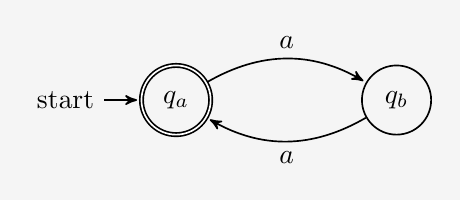
\begin{tikzpicture}[->,>=stealth',shorten >=1pt,auto,node distance=2.8cm,
	semithick]
	\node[initial,state,accepting]   (A)                      {$q_a$};
	\node[state]           (B)  [right of=A]  {$q_b$};
	
	\path (A) edge [bend left]             node {$a$} (B)
	(B) edge [bend left]              node {$a$} (A);
	\end{tikzpicture}}

\vspace{0.5em}

\end{MyMdframed}

\end{figure}

A simple DFA that accepts a number $2n$ of the character \texttt{a} is shown in figure \ref{figure:dfa:1}. We can define $M = (\{q_a,q_b\}, \{a\}, \delta, q_a, \{q_a\})$ and informally describe the transition function $\delta$ as mapping $(q_a, 'a') \rightarrow q_b$ and $(q_a, 'a') \rightarrow q_a$. The automaton alternates between states $q_a$ and $q_b$ every time a new character is processed -- whist the length is even, $q_a$ will be active and the string will be considered in the language.

Non-deterministic finite automata are equivalent in language recognition ability to the DFAs discussed above, but use a different processing model \citep[p.~46]{sipser2012introduction}. There is no requirement to account for every possible character from the alphabet $\Sigma$ and there is a new concept of an epsilon transition which can always be followed; such a transition is depicted by an edge labelled $\epsilon$ in automata diagrams. NFAs can be thought of as being able to process multiple ``paths'' in parallel. Figure \ref{figure:nfa:1} illustrates an NFA using $\epsilon$-transitions to capture \emph{alternation}.

We can formalise the definition of an NFA in terms of a 5-tuple $(Q, \Sigma, \delta, q_0, F)$ where the elements of the tuple are described below. Note that the transition function has changed.

\begin{description}
\item[$Q$] The set of states in the automaton.
\item[$\Sigma$] A set of characters known as the \emph{alphabet}.
\item[$\delta$] Table defining \emph{transitions} between states. Formally, it can be described as a function $\delta : Q \times \Sigma \cup \{\epsilon\} \rightarrow \mathcal{P}(Q)$ -- given a state from $Q$ which the automaton is in, receiving the character in $\Sigma$ will result in a set of possible new states, derived from the powerset (set of possible subsets) of $Q$.
\item[$q_0$] The initial state which the automaton starts in.
\item[$F$] The set of accepting states.
\end{description}

Not all languages are regular. For example, the matching parentheses language which accepts strings such as \texttt{(())} but not \texttt{(}, \texttt{))} or \texttt{((())} can be proven non-regular by contradiction (using the pumping lemma described in \citet{rabin1959finite}). As a result, no DFA, NFA or regular expression\footnote{The language \emph{can} however be recognised using a pushdown automata because it belongs to the set of deterministic context-free languages.} can encode the rules of this language.




\begin{figure}[H]
	\begin{MyMdframed}
	\vspace{0.5em}
 

\caption{\label{figure:nfa:1} An NFA, representing the language \texttt{g+|f+}}
\vspace{0.5em}
\captionsetup{style=default}

		\makebox[\linewidth][c]{\centering 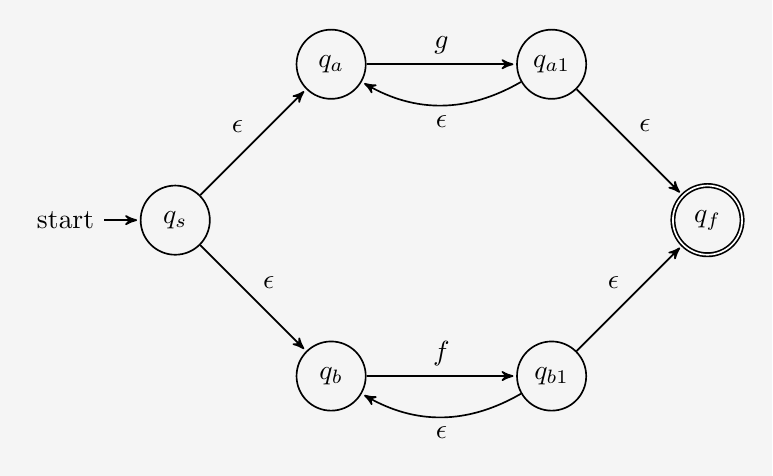
\begin{tikzpicture}[->,>=stealth',shorten >=1pt,auto,node distance=2.8cm,
		semithick]
		\node[initial,state]   (A)                      {$q_s$};
		\node[state]           (B)  [above right of=A]  {$q_a$};
		\node[state]           (B1) [right of=B]        {$q_{a1}$};
		\node[state]           (C)  [below right of=A]  {$q_b$};
		\node[state]           (C1) [right of=C]        {$q_{b1}$};
		\node[state,accepting] (F)  [below right of=B1] {$q_{f}$};
		
		\path (A) edge              node {$\epsilon$} (B)
		(A) edge              node {$\epsilon$} (C)
		(B) edge node {$g$} (B1)
		(B1) edge [bend left] node {$\epsilon$} (B)
		(B1) edge node {$\epsilon$} (F)
		(C) edge node {$f$} (C1)
		(C1) edge [bend left] node {$\epsilon$} (C)
		(C1) edge node {$\epsilon$} (F);
		\end{tikzpicture}}
		
\vspace{0.5em}

The initial state is $q_0$. As this automaton is non-deterministic, it can be viewed as ``branching'' and entering the two states $q_a$ and $q_b$ due to the $\epsilon$-transitions. $q_a$ is used for the \texttt{g+} component of the alternation in the original regular expression and, similarly, $q_b$ is used for the \texttt{f+} component. Both of these states require at least one occurrence of their respective character before entering the $q_{x1}$ state ($x in \{a, b\}$) -- the only way to proceed to the final accepting state $q_f$. 

\vspace{0.5em}

\end{MyMdframed}
\end{figure}

\subsection{Programming Language Support}

Most programming languages include a regular expression engine and offer syntax inspired by Perl's regular expressions. These ``regular'' expressions are often more powerful than the formal regular expressions discussed previously and can match non-regular languages.

For example, recall the balanced parentheses language. In PCRE (a library providing a regular expression engine inspired by Perl), the \texttt{(?n)} pattern can be used to recursively match using the n\textsuperscript{th} capture group. It is possible to then write an expression which will match balanced parentheses. Micosoft's .NET platform includes an extension to support \emph{balancing group definitions} which would also allow for balanced parentheses to be matched. Regular expressions using these language features and extensions are \emph{regular} in the formal sense. Throughout this project, we only consider regular expressions according to their formal definition.

\section{SAT and SMT Solvers}

\subsection{Introducing SAT}

The SAT decision problem involves a propositional Boolean logic formula built from a number of variables and operations conjunction $\land$, disjunction $\lor$ and negation $\neg$. The question concerns whether the formula is \emph{satisfiable}--i.e. is there a set of \emph{valuations} for each of the variables which results in the overall formula evaluating to true?

If a formula \emph{cannot} be satisfied, there is no valuation for which the formula will evaluate to true. For example, the clauses may contradict each other as in $(a) \land (\neg a)$. Example \ref{example:sat:1} shows a satisfiable formula comprising 2 clauses and 3 variables; example \ref{example:sat:2} shows, by exhaustive evaluation, a problem which cannot be satisfied.



\begin{example}{A simple SAT problem, with satisfying valuation}
 Can the \(
			(a \lor b \lor c) \land (\neg b \lor c)
		\) propositional logic formula be satisfied?\\
		
		\textcolor{id7-emerald-green}{\textbf{Yes}}, set $a = T$, $b=F$, $c=T$. Then clause 1 evaluates to $(T \lor F \lor T) = T$ and clause 2 evaluates to $(\neg F \lor T) = T$. The whole formula evaluates to $T \land T = T$.
\vspace{0.5em}
\label{example:sat:1}
\end{example}


\begin{example}{A formula which cannot be satisfied}
	Can the \(
	(a \lor b) \land (\neg a \lor b) \land (\neg b)
	\) propositional logic formula be satisfied?\\
	
	\textcolor{id7-ruby-red}{\textbf{No}}, the clauses are contradictory. The table below shows exhaustively that no valuation of the variables result in the formula evaluating to true:
	
	\arrayrulecolor{lightgrey} % <---
	\def\arraystretch{1.5}%  1 is the default, change whatever you need
	\begin{table}[H]
		\centering
		\rowcolors{1}{}{lightgrey}
		\begin{tabular}[t]{|p{0.05\linewidth}|p{0.05\linewidth}|p{0.1\linewidth}|}
			\hline
			\rowcolor{id7-aubergine}
			{\color[HTML]{FFFFFF} $\mathbf{a}$} & {\color[HTML]{FFFFFF} $\mathbf{b}$} & {\color[HTML]{FFFFFF} \sffamily  \textbf{Result}} \\ \hline
			$F$ & $F$ & $F$  \\ \hline
			$F$ & $T$ & $F$  \\ \hline
			$T$ & $F$ & $F$  \\ \hline
			$T$ & $T$ & $F$  \\ \hline
		\end{tabular}
		\caption{Enumerating all possible valuations for the variables $\{a, b\}$ used in the formula.}
		\label{table:landingredesign}
	\end{table}
\label{example:sat:2}
\end{example}


\subsubsection{Normal Forms}

Examples of formulae up to this point have been given in \emph{Conjunctive Normal Form} (CNF). That is, they are provided as a conjunction of disjunctive clauses. It is possible to convert any Boolean logic formula into this form. To \emph{evaluate} a given formula using a valuation of Boolean variables and values, we simply consider each clause in turn and enumerate the literals within each clause. Once any one literal has been found to be true, the disjunctive nature of the clauses allows us to ignore any remaining terms and move onto the next. Similarly we can skip all remaining clauses if one clause in a CNF formula is found to evaluate to $F$, since all clauses must be true.

To solve SAT, we could devise a naïve algorithm considering all possible assignments and evaluating the formula at each stage (as we did in example \ref{example:sat:2}). Clearly such an approach would be inefficient--for Boolean variables with two possible assignment values, this algorithm would work in $\mathcal{O}(2^n)$.

As discussed in \citet{miltersen2005converting}, it is also possible to convert formulae to \emph{Disjunctive Normal Form} (DNF) using De Morgan's law. Example \ref{example:sat:3} illustrates the conversion process. This is of some note, because SAT restricted to formulae in DNF can be solved in linear time using the procedure below:


\begin{outline}
	\1 For each clause in the formula, check each literal and keep a note of whether it is negated or not

	\2 If a clause contains the same literal and its negation, mark the clause as unsatisfiable.
	\2 Otherwise, the clause can be satisfied. The valuation for each literal is $F$ if they are negated, and $T$ otherwise.

	\1 If at least one clause is satisfiable, the entire problem is -- and we can stop processing.
	\1 If no clauses are satisfiable, the problem cannot be satisfied.
\end{outline}

\begin{example}{Conjunctive and disjunctive normal forms}
	Here we use the formula from example \ref{example:sat:1} and show the DNF equivalent:
	\begin{description}
		\item[CNF] \(
		(a \lor b \lor c) \land (\neg b \lor c)
		\)
		\item[DNF] \(
		(a \land \neg b) \lor (c)
		\)
	\end{description}

\spacedrule{}

	A more interesting example might comprise a formula of structure  \(
	(a \lor b) \land (c \lor d) \land (e \lor f)
	\), which can be converted to the DNF formula below:
	
	\[
	(a \land c \land e) \lor (a \land c \land f) \lor (a \land d \land e) \lor (a \land d \land 
	f) \lor (b \land c \land e) \lor (b \land c \land f) \lor (b \land d \land e) \lor (b \land d \land
	f)
	\]
\vspace{0.25em}
\label{example:sat:3}
\end{example}

However, as the second formula in example \ref{example:sat:3} illustrates, there can be an \emph{exponential increase} in size for an arbitrary propositional logic formula written in CNF. Hence, in the general case, we cannot use this conversion procedure to solve SAT in linear time for any Boolean logic formula.

\subsection{Cook-Levin and NP Completeness}

SAT is NP complete. It is computationally straightforward (i.e. possible in linear time) to check if a given valuation of variables is satisfying by evaluating the entire formula. Furthermore, it has been shown that any problem in NP can be reduced to SAT by way of a nondeterministic Turing machine encoding \citep{Cook:1971:CTP:800157.805047} -- this is the statement of the Cook-Levin theorem.

This has an impact on the practical application of SAT solvers and the reliability of such applications. Whilst heuristics can be used to efficiently solve some SAT problems, there is no guarantee that a particular problem will be able to be solved in a reasonable timeframe.


\begin{algbox}{Knuth's SAT0}

First discussed in \citet{Knuth:2015:ACP:2898950}, \citeauthor{Knuth:2015:ACP:2898950}'s \emph{Algorithm A} solves SAT by backtracking. Designed as a basic solution to the problem of designing a SAT solver, it is an improvement on the naïve algorithm discussed earlier. For a SAT problem involving $n$ variables, the algorithm proceeds by setting the $n$\textsuperscript{th} variable to its ``most plausible'' value and then recursively doing the same for the $n-1$ previous variables. If at any point a contradiction is encountered, the value assigned to $n$ is flipped and the process repeats. For literals which are never negated in any clause, we can assume that they are true without issue. These are known as ``pure literals'', a concept which reappears in the DPLL algorithm discussed later.

At each stage, clauses must be modified to take into account the assignments, such as $x_1 = T$. This is achieved by removing any \emph{clause} which contains a literal $l = x_1$. For any clauses containing $l = \neg x_1$, this literal must be removed because it can no longer be used to satisfy the clause now that $x_1$ has been set. If $x_1$ is set to $F$, the same procedure happens in reverse (clauses containing $l = \neg x_1$ are removed, literals requiring $l = x_1$ are removed).
\label{algorithm:knuth:sat0}
\end{algbox}
\subsection{DPLL}

A more advanced approach than Knuth's SAT0 (discussed in algorithm \ref{algorithm:knuth:sat0}) is the \emph{Davis–Putnam–Logemann–Loveland} (DPLL) algorithm. DPLL underpins a number of modern SAT solving software such as Microsoft's \emph{Z3} where it powers the core theory solver \citep{de2008z3}. The algorithm was developed by improving on the DP algorithm which was published in 1960 in \citet{Davis:1960:CPQ:321033.321034}.

For an arbitrary CNF SAT problem, the algorithm uses a process known as \emph{unitary resolution}. If all previous variables in a CNF clause are false, the disjunctive nature implies that the last literal \emph{must} be true. DPLL applies this process recursively. As briefly mentioned in algorithm \ref{algorithm:knuth:sat0}, DPLL also uses the concept of a ``pure literal'' which is defined as a literal for which its negation does not appear in the Boolean formula.



\subsection{Satisfiability Modulo Theories (SMT)}

\subsection{DPLL(T): Extending DPLL to Arbitrary Theories}

\section{Static Analysis}

\section{Parsing}

\chapter{Prior Art}

There is a wealth of existing work within the areas of static analysis and program verification. This chapter aims to explore and evaluate some of the these works.

\section{Program Verification}

\subsection{Dafny}

Dafny is a language designed by Microsoft Research with built-in static verification functionality and modern programming language features. The language itself is imperative and allows programmers to specify functions with pre and post-conditions which are verified at compile time \citep{dafny2}. Recent versions of Dafny allow programs to be compiled into executables targetting the .NET framework \citet{dafny}.

The language uses an intermediate representation language known as \emph{Boogie} which is able to derive constraints. These constraints are passed to the Z3 SMT solver to verify the user's program.

\begin{mycode}{csharp}{Factorial function and a pre-condition violation}{Dafny}
function Fac(n: int): int
requires n >= 1 // pre-condition
{
	// base case          recursion
	if n == 1 then 1 else n * Fac(n - 1)
}

function Main(): int
{
	Fac(-2) // violation
}
\end{mycode}

\subsection{LiquidHaskell}

\section{Static Analysis and Security Tooling}

\subsection{Roslyn Security Guard}

\subsection{Snyk}

\chapter{Design and Implementation}

\chapter{Testing}

\chapter{Evaluation and Conclusions}

\section{}

\chapter{Future Work}


\titleformat{\chapter}[display]
{\normalfont \sffamily \Huge  \color{id7-aubergine}}
{}{0pt}{}[]

\bibliographystyle{agsm}
\bibliography{bibliography}

\end{document}
